%------------------------------------------------------------------------------------------%
%------------------------------------------------------------------------------------------%
%------------------------------------------------------------------------------------------%
%                                      FILE BEGINS
%------------------------------------------------------------------------------------------%
%------------------------------------------------------------------------------------------%
%------------------------------------------------------------------------------------------%

%------------------------------------------------------------------------------------------%
%------------------------------------------------------------------------------------------%
%                                    DOCUMENT CLASS
%------------------------------------------------------------------------------------------%
%------------------------------------------------------------------------------------------%
\documentclass[a4paper]{jpconf}

%------------------------------------------------------------------------------------------%
%------------------------------------------------------------------------------------------%
%                                       PACKAGES
%------------------------------------------------------------------------------------------%
%------------------------------------------------------------------------------------------%
\usepackage{booktabs}
\usepackage{cite}
\usepackage{float}
\usepackage{graphicx}
\usepackage[caption=false]{subfig}

%------------------------------------------------------------------------------------------%
%------------------------------------------------------------------------------------------%
%                                    DOCUMENT BEGINS
%------------------------------------------------------------------------------------------%
%------------------------------------------------------------------------------------------%
\begin{document}

%------------------------------------------------------------------------------------------%
%                                        HEADER
%------------------------------------------------------------------------------------------%

\title{The Fiber-Matrix Interface Crack Problem and its Solution by the Finite Element Method}

\author{\underline{Luca Di Stasio}$^{1,2,a}$ , Janis Varna$^{2,b}$ and Zoubir Ayadi$^{1,c}$ }

\address{$^{1}$SI2M, IJL, EEIGM, Universit\'e de Lorraine, 6 Rue Bastien Lepage, F-54010 Nancy, France\\$^{2}$Division of Polymer Engineering, Lule\aa\ University of Technology, SE-97187 Lule\aa , Sweden }

{\vspace*{5pt}\address{E-mail: $^{a}$luca.di-stasio@univ-lorraine.fr, $^{b}$janis.varna@ltu.se, $^{c}$zoubir.ayadi@univ-lorraine.fr}}
%\address{$^{a}$luca.di-stasio@univ-lorraine.fr}, \address{$^{b}$janis.varna@ltu.se}, \address{$^{c}$zoubir.ayadi@univ-lorraine.fr}

%------------------------------------------------------------------------------------------%
%                                       ABSTRACT
%------------------------------------------------------------------------------------------%

\begin{abstract}
Crack initiation in thin-ply laminates has been mostly neglected and still represents a field ripe for investigation. Understanding is still lacking about the dependence of energy release rate with respect to debond size and position, adjacent plies’ orientation and thickness. Furthermore, the influence of fiber volume fraction, material selection, boundary conditions, load type and distribution should be considered in order to grasp the inner workings of this phenomenon. Detailed knowledge of the mechanisms underlying the initiation of fracture inside a single ply is useful in a twofold way: from the designer’s perspective, by providing guidelines on optimal laminate design; from the modeler’s perspective, by highlighting the best strategies to simulate crack initiation in terms of solver selection, mesh quality, boundary conditions, load type and distribution. To address these issues, several 2-D models of Representative Volume Elements (RVEs) have been developed by combining together different variations of these building-blocks. Computed crack shapes are analyzed; energy release rates are computed for different debond size, as well as FE solver performances to evaluate their dependence on mechanical parameters.
\end{abstract}

%------------------------------------------------------------------------------------------%
%                                     INTRODUCTION
%------------------------------------------------------------------------------------------%

\section{Introduction}
\subsection{Contemporary trends in the development of FRPC laminates}
In the last 40 years, pressure has been growing on the transportation industry to increase efficiency and reduce fuel consumption. If the two energy crises of 1973 and 1979 focused the attention of the industry on the need for efficient fuel usage, it is today the growing concern on climate change and pollution, enshrined in the Paris agreement of December 2015, that is pushing for the adoption of innovative technologies to reduce the emissions of $CO_{2}$ and pollutants. Although the issues of concern have been changing over the decades, the directions of innovation remain the same: on one side, the search for new propulsive technologies and the optimization of existing ones; on the other hand, the development of innovative materials to reduce structural weight without compromising integrity and safety.\par
In the latter line of research, proper to materials scientist and engineers, Fiber Reinforced Polymer Composites (FRPC) laminates have been proven to be optimal substitutes for metals, which dominated both the transportation and the construction industry since the dawn of the Second Industrial Revolution in the XIX century. Indeed, FRPCs offer high mechanical properties with a significant reduction in weight, giving them a high competitive advantage in structural application where high thermal loads and very corrosive environment are absent. Furthermore, their very nature as composites provides the designer with the possibility of tuning their properties and performances by changing the structure and mutual interconnections of its phases at different scales. Nonetheless, major problems exist with respect to damage tolerance: materials employed have typically a brittle behavior, which often leads to unstable fracture propagation and sudden failure. Damage in conventional FRPC laminates usually originates in off-axis plies by transverse cracking in the matrix at or close to fiber surfaces; it then spreads across the width of the ply and induces delaminations between adjacent plies; finally, fibers' failure is shortly followed by the component's collapse. Due to its microscopical origin, timely detection of damage onset is difficult and hard to achieve, adding another criticatility to the application of composite laminates.
\subsection{The Spread Tow Technology}
Research has thus focused on the development of techniques, be they technological, experimental, analytical or numerical, to further reduce weight and to increase the tolerance to damage in FRCP laminates. One main direction of technological progress has focused on the concept of \textit{thinning}, i.e. the production of ever thinner plies, leading to the development of what is nowadays known as the \textit{spread tow technology}. Conventionally, fibers are produced as bundles or \textit{tows} comprising at least $12/24k$ filaments; tows are then stacked together and impregnated in order to produce prepreg plies. At the heart of the \textit{spread tow technology} lies the idea of opening or \textit{spreading} such tows to create thinner and wider tapes, to be then used in the production of unidirectional (UD) prepregs or woven fabrics. First attempts to turn the idea into practice date back to the 1970's~\cite{spreadtowpatent:1974}, when a Venturi injector opposite to the fibers' pulling direction was employed to split the tow. Other methodologies were then proposed, applying mechanical~\cite{spreadtowpatent:1991,spreadtowpatent:1992,spreadtowpatent:2000} and electrostatic techniques~\cite{spreadtowpatent:1993}. Nonetheless they all suffered the same drawbacks: widespread fibers' breakages and deterioration of fibers' surface properties, in particular their wettability. A breakthrough arrived around the turn of the millenium with the development at the Fukui Prefecture's Industrial Technology Center in Japan of a new spreading technique~\cite{KawabeTomodaMatsuo:1997,spreadtowpatent:2003,Kawabe:2008,SasayamaTomoda:2009}, based on the combined use of focused air jets and a vacuum pump perpendicular to the pulling direction of fibers. Thanks to its capacity of avoiding fiber breakage and fiber's surface property loss, this technology has been recently been applied on industrial scale to produce high-quality extremely thin fiber-reinforced prepreg plies. The few manufacturers of this kind of composite material, such as North Thin Ply Technology \cite{ntpt} in Switzerland and Oxeon \cite{oxeon} in Sweden, are nowadays capable of providing prepregs with thicknesses up to 2-4 times the reinforcement's diameter for high performance carbon and glass E fibers.
\subsection{The Thin Ply Effect}
Experimental studies~\cite{SihnKimKawabeTsai:2007,SaitoTakeuchKimpara:2012,ArteiroCatalanottiXavierCamanho:2013,AmacherCugnoniBotsisSorensenSmithDransfeld:2014} have shown that the use of thin plies in cross- and angle-ply laminates is beneficial in terms of increased mechanical performance and improved tolerance to damage with concurrent savings in weights. The key factor underpinning the success of this technology is a phenomenon first experimentally observed around 40 years ago~\cite{ParviziBailey:1978,BaileyCurtisParvizi:1979}, which have come to be known as the \textit{thin ply effect} in the composite community. The main observation is that the transverse strength at failure measured for unidirectional composites (UD) is not applicable to a thin layer inside a laminate. Its real strength, known as the \textit{in-situ strength}, is in fact much higher~\cite{FlaggsKural:1982} as shown in Figure~\ref{fig:insitustrength}.\par
\begin{figure}
\begin{center}
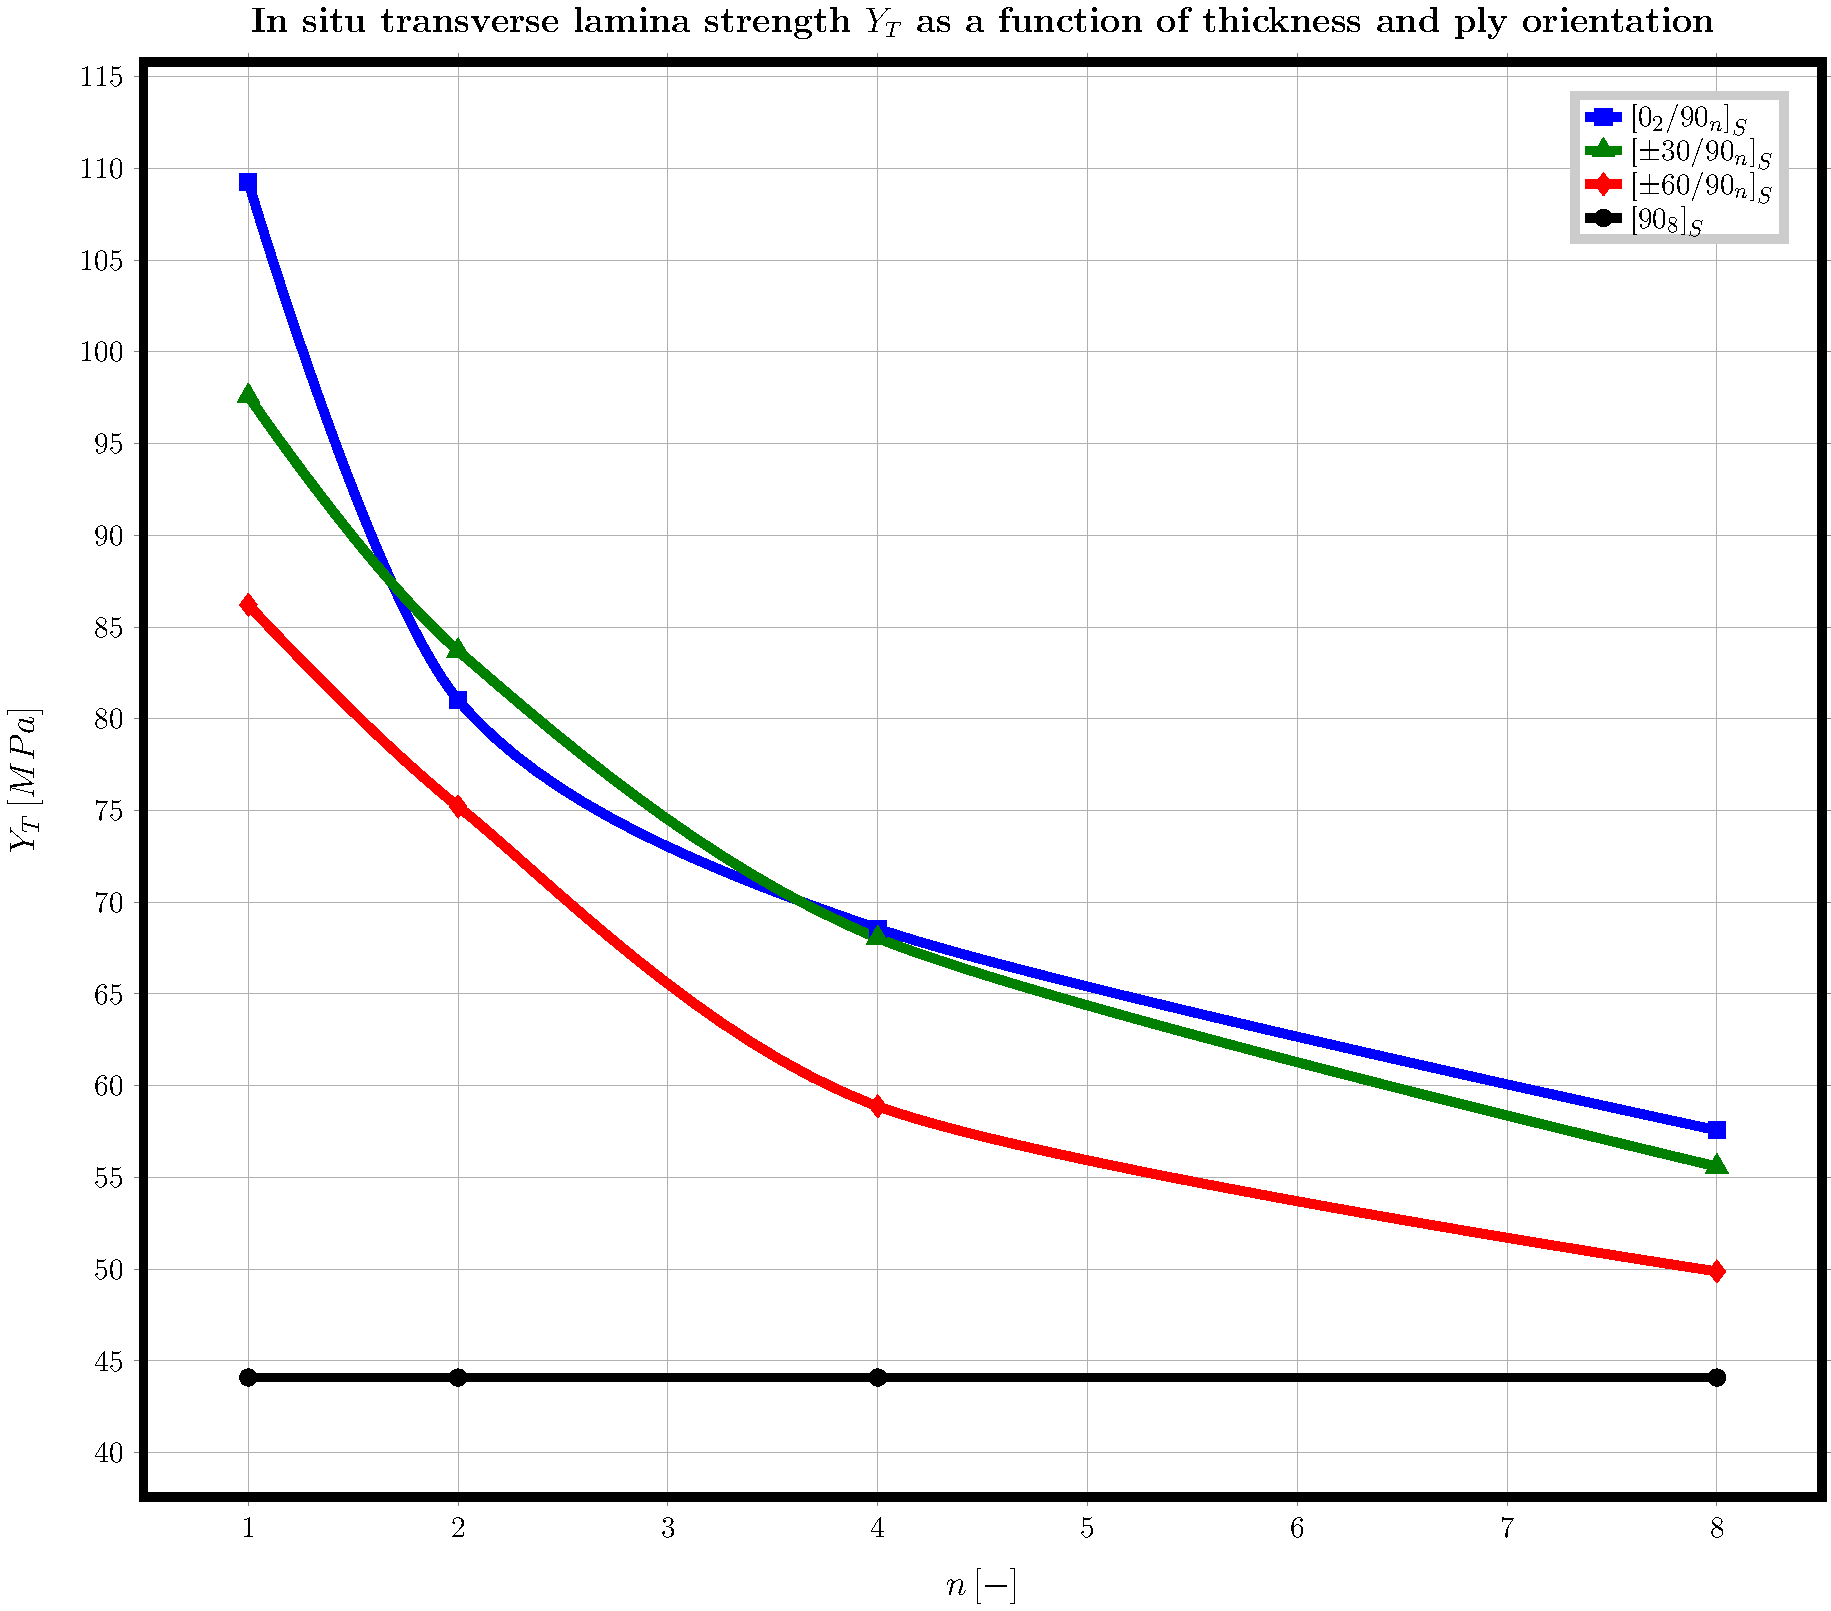
\includegraphics[height=0.4\textheight]{Flaggs-Kural_InSituTransverseStrength.pdf}
\end{center}
\caption{\label{fig:insitustrength}Measurements of in-situ transverse lamina strength $Y_{T}$ with respect to ply thickness and orientation from~\cite{FlaggsKural:1982}. In black, results for an UD $\left[90_{8}\right]_{S}$ laminate; in blue, $\left[0_{2}/90_{n}\right]_{S}$; in green, $\left[\pm30/90_{n}\right]_{S}$; in red, $\left[\pm60/90_{n}\right]_{S}$. The thickness of the transverse ply is represented by $n$, which is the number of prepreg laminae comprising the ply in the stacking sequence of the laminate.}
\end{figure}
Modeling of thin plies have mostly focused on the development of homogenized material behaviors to be applied at the lamina or laminate level. In~\cite{AmacherCugnoniBotsisSorensenSmithDransfeld:2014}, the authors firstly develop a macroscopic model based on Classical Laminate Theory (CLT) to compute the firts-ply failure and ultimate strength with the application of the Tsai-Hill failure criterion; then, they develop a phenomenogical calculation strategy based on the in-situ strength model presented in~\cite{CamanhoDavilaPinhoIannucciRobinson:2006} to evaluate the ultimate strength's scaling in thin plies. A different strategy is adopted in~\cite{SaitoTakehuchiKimpara:2014}, where a plane-strain model is developed and analyzed by means of the Finite Element Method (FEM) for different thicknesses. The model is built to be representative of the entire laminate but to directly consider elasto-plastic and damage mechanisms in the transverse ply. The authors thus consider a rectangular element comprising a central $90^{\circ}$ ply bounded on the north and south side by two homogenized $0^{\circ}$ layers, with symmetry boundary conditions on the north and west side and controlled in displacement by means of an applied strain. A generic system of a in-plane isotropic fiber sorrounded by an isotropic matrix is adopted. Decohesion at the fiber/matrix interface is represented by means of cohesive elements and thermal effects are modeled by means of an initial residual stress state. An analoguos work is presented in~\cite{HerraezMoraNayaLopesGonzalezLLorca:2015}, where the authors present a similar FEM model based on a Representative Volume Element (RVE) of a thin cross-ply laminate. They choose to use periodic boundary conditions to represent the repeating character of the RVE and to adopt multiple materials: AS4 carbon and E glass for fibers, and Hexply resin 8552 from Hexcel and MTM57 resin from Advanced Composite Group for the matrix. By showing the good adherence of numerical crack morphologies to microscopic observations, both works have shown the possibilities provided by the Finite Element Method in the contest of damage propagation analysis. However, their approach suffer from two major shortcomings. Firstly, crack initiation is not studied and cannot be precisely identified: by analysing a large set of fibers, the effect of factors like volume fraction, initial debond position and size, position and size of neghboring fibers, boundary conditions and bounding plies characteristics cannot be distinguished and assessed. Furthermore, damage propagation-based models recast the complexity of the phenomenon into a greater set of material parameters, such the critical energy release rates and maximum stresses at fiber/matrix interface. Unfortunately, several of these are inaccessible to the experimenter and thus cannot be reliably measured. Indirect methods of estimation have been proposed, as for example in~\cite{CanalGonzalezSeguradoLLorca:2012}, but the applicability of such parameters outside the domain of training is still an open question.\par
\subsection{Objectives and Approach}
On the other hand, investigation of crack initiation at the microscopic level in thin plies has been mostly neglected and still represents a field ripe for investigation. Understanding is still lacking about the dependence of energy release rate with respect to initial flaws geometry, material selection, laminate geometry and stacking sequence. A law of the type
\begin{equation}
\label{eq:energyreleasetype}
G_{*c}=G_{*c}\left(\theta_{debond},\Delta\theta_{debond}, E_{\left(\cdot\cdot\right)}, \nu_{\left(\cdot\cdot\right)}, G_{\left(\right)},VF_{f}, t_{ply}, \frac{t_{ply}}{t_{bounding\ plies}}\right)
\end{equation}
is still missing from the toolbox of the composite designer. Even the number and type of independent parameters in Equation~\ref{eq:energyreleasetype} are at present nor clearly defined neither completely explored. The results of such investigation are beneficial in a twofold way: they can provide guidelines on laminate design for enhanced damage tolerance, and they could offer insights on the best method of simulation with the respect to choice of solver selection, mesh quality, boundary conditions, load type and distribution. In order to explore this vast and mainly unexplored area of knowledge, the use of Representative Volume Elements (RVEs) has been deemed the best tool for the task at hand. By creating several RVEs with different features and conducting parametric studies varying initial debond position and size, the effect of each different parameter can be isolated and analyzed correctly.

%----------------------------------------------------------------------------------------------%
%  MICROMECHANICAL MODELING WITH REPRESENTATIVE VOLUME ELEMENTS
%----------------------------------------------------------------------------------------------%

\section{Micromechanical modeling with Representative Volume Elements (RVEs)}
\subsection{Introduction to Representative Volume Elements}\label{sub:introRVE}
The concept of Representative Volume Element was first introduced by Hill~\cite{Hill:1963} for the evaluation of the macroscopic elastic properties of multiphase reinforced solids and it has been shown to be a useful tool for elastic calculations in Fiber Reinforced laminates as well~\cite{SunVaidya:1996}. In general, a Representative Volume Element should be constructed to represent with sufficient accuracy the details of the microstructure while being representative of the overall body in a statistical sense, i.e. the volume averages of stress and strain fields over the RVE and the overall body should be the same~\cite{Hashin:1983}. In the case of elastic modeling of composites, the definition of the correct RVE is linked to a macroscopic mathematical formulations, based on variational or mean-field approaches~\cite{Hashin:1962,Hashin:1963}. However, when it comes to non-linear material behavior such as damage, non-linear elasticity and plasticity, the construction of Representative Volume Elements becomes difficult and less defined. In~\cite{SwaminathanGhoshPagano:2006,SwaminathanGhosh:2006} a method for RVE design is proposed based on statistical equivalence. In~\cite{BulsaraTalrejaQu:1999} the optimal size for a UD RVE with multiple fibers is searched by means of numerical simulations.\par
In the present work, a different approach is proposed. Instead of deriving it from a mathematical model, be it variational or statistical, the RVE is considered to be constructed upon a series of building-blocks, each one offering different choices. Different Representative Volume Elements can be built and subsequently analysed by means of the Finite Element Method. Numerical simulations are thus used not to solve analytical problems for which closed-form solutions are not available, but to perform numerical experiments, in analogy to experiments in the laboratory, to be compared with physical observation in order to draw conclusions on the assumptions made. This method takes inspiration from the Computational Statistical Physics field~\cite{Krauth:2009,HoffmannSchreiber:2002}, where numerical simulations based on simple rules (Ising model, Potts model, cellular automata) are used to analyze physical problems not thorugh the discretization of analytical models, but on a process of \textit{trial and error} or \textit{numerical experimentation}. In this way, not only the dependence on the crack initiation process on geometric and material parameters can be investigated, but also conclusions on the design of RVEs in the presence of damage can be drawn. Some interesting questions can be addressed by the application of the explained method:
\begin{itemize}
\item How does the energy release rate for a debond at the fiber/matrix interface in a thin ply depend on crack geometry, material choice, thin ply's and bounding plies' thicknesses and laminate stacking sequence?
\item What is the minimum number of fibers to correctly model the onset of transverse cracking in thin plies?
\item How does the result depend on the choice of boundary conditions? Can the effect of the bounding plies be modeled by a set of equivalent boundary conditions?
\item What is the effect of the type of load, i.e. applied strain (displacement controlled) with respect to applied stress (force controlled)?
\end{itemize}
\subsection{Design of Representative Volume Elements}
For the design of Representative Volume Elements for the investigation of transverse cracking in thin-ply laminates, the following building blocks or characteristics are identified:
\begin{enumerate}
\item space dimensionality: 2D, quasi-3D (3D shells) or full 3D;
\item stacking sequence;
\item structural assumptions: plane strain, plane stress or none;
\item material system;
\item crack type: interface debond, matrix crack or both;
\item damage modeling: Linear Elastic Fracture Mechanics (LEFM) with repsect to Cohesive Zone Modeling (CZM);
\item fiber/matrix interface behavior: contact interaction, cohesive interaction or continuity constraints on displacements;
\item load control: displacement or force;
\item boundary conditions.
\end{enumerate}
By fixing the first 8 variables and keeping the last one free, it is now possible to construct different RVEs distinguishes by a different choice of boundary conditions. Let us start by considering a generic thin-ply laminate and by modeling it as a 3D plate, see Figure~\ref{fig:macrotomicro}. The $x,\underline{i}$ axis is parallel to the laminate $0^{\circ}$ direction. We consider a generic section $x-z$ of the laminate far from the edges and we focus on the thin transverse ply. We assume the section to be 2-dimensional and subjected to plane-strain conditions. Furthermore, we assume the stacking sequence to be $\left[0,90,0\right]$: the thin transverse ply is the one at $90^{\circ}$, placed at the center of the laminate and bounded by two identical $0^{\circ}$ plies. Boundary conditions will thus be the same on the north and south sides of the RVE. Having fixed the first 3 variables, we consider a generic single fiber in the ply together with its sorrounding matrix and we extract a square element around the fiber. The half-length $l$ of the side is determined with respect to the fiber radius $R_{f}$ and fiber volume fraction $VF_{f}$:
\begin{equation}
l=\frac{1}{2}R_{f}\sqrt{\frac{\pi}{VF_{f}}}.
\end{equation}
We assume the load to be controlled in displacement, applied on the east and west side of the element and equal to the applied strain $\bar{\varepsilon}_{xx}$, which is considered to be equal to $1\%$.
\begin{figure}[H]
\centering
   \subfloat[Free boundary conditions.\label{subfig:free}]{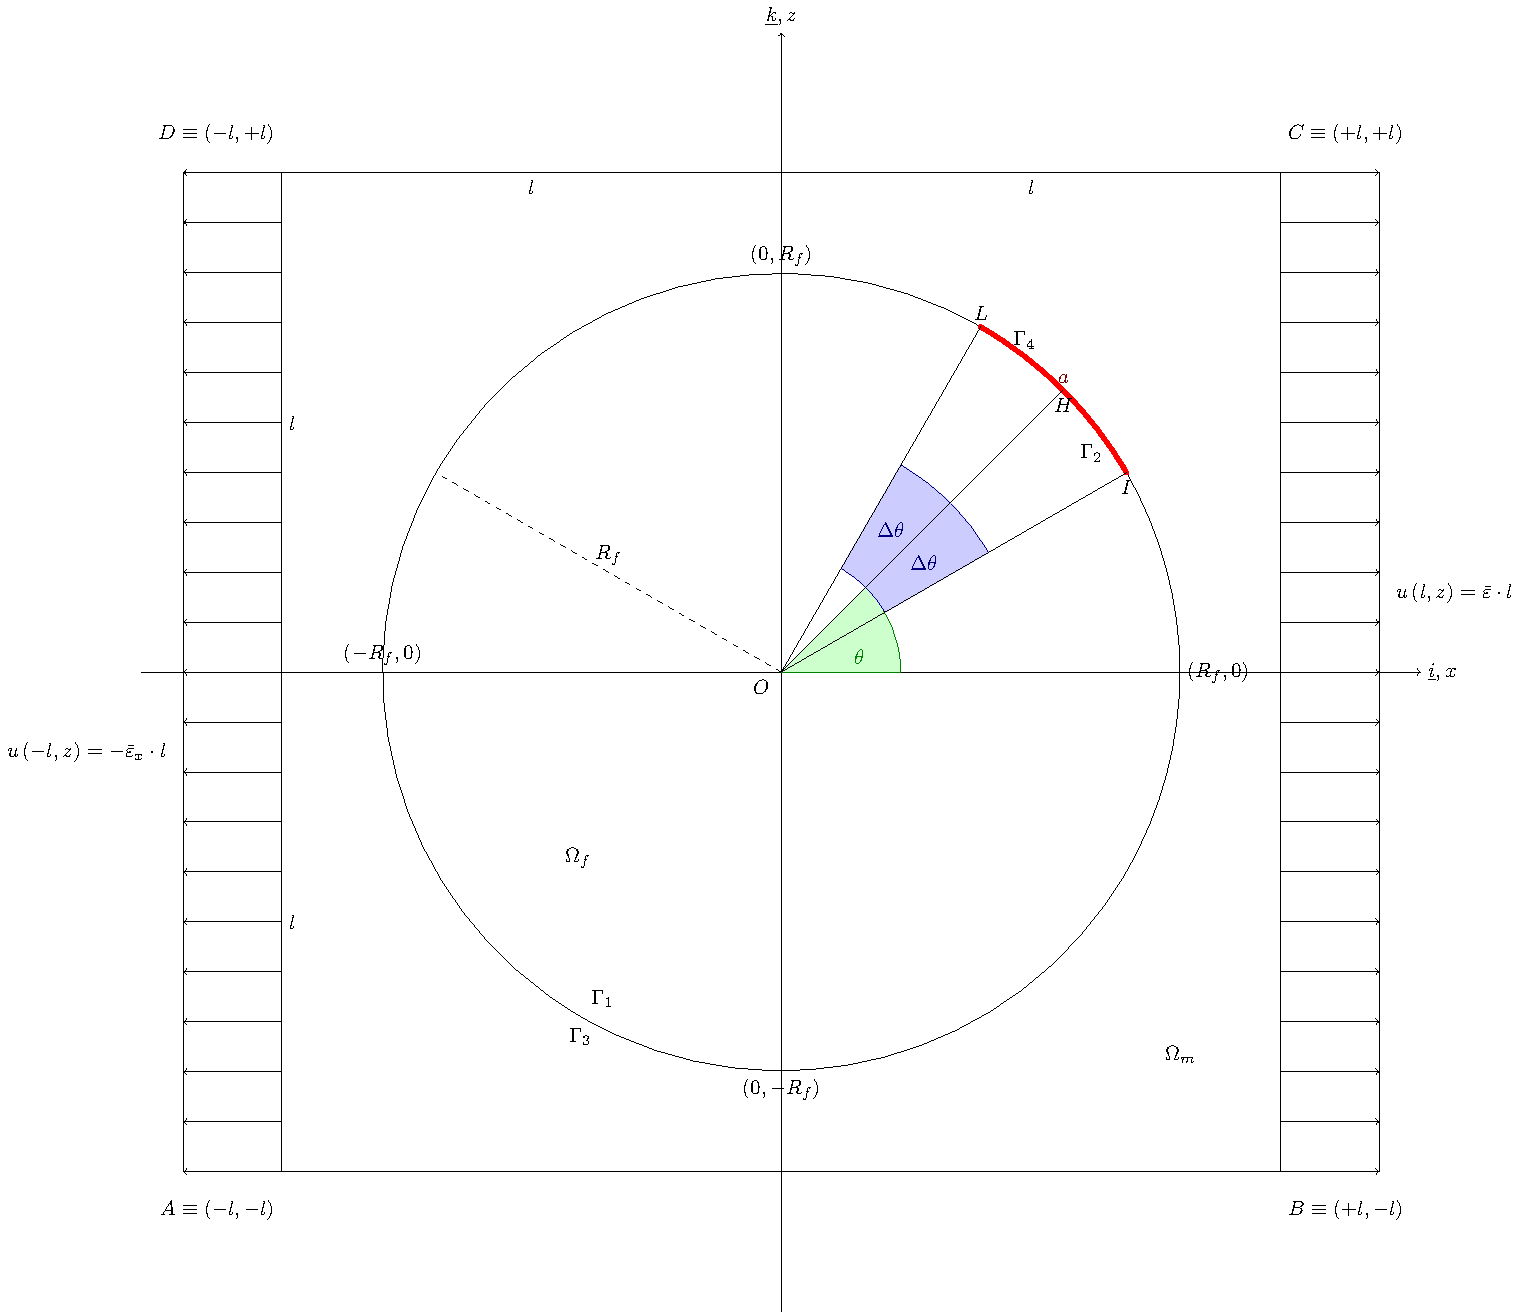
\includegraphics[height=0.275\textheight]{LEFM2DsRVEsFsDfreeBCULappAxialDispLR.pdf}}\\
\subfloat[Above: constant vertical displacement. Below: homogeneous boundary conditions.\label{subfig:homo}]{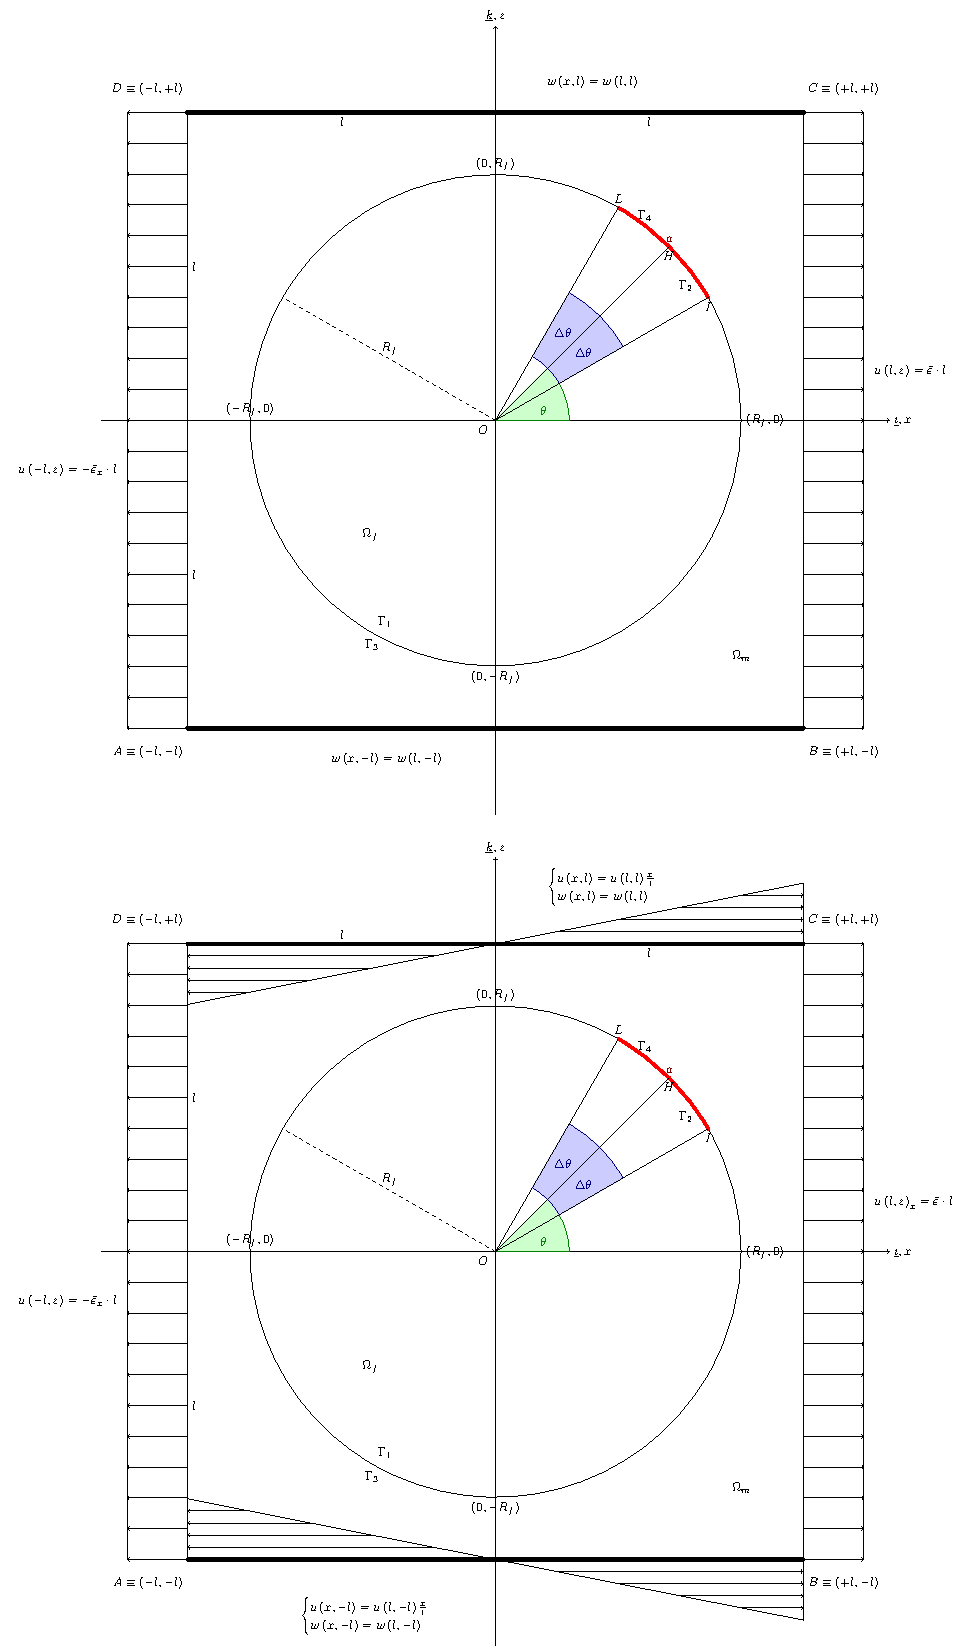
\includegraphics[height=0.275\textheight]{singleRVEs.pdf}}\quad\subfloat[Bounded RVE.\label{subfig:bounded}]{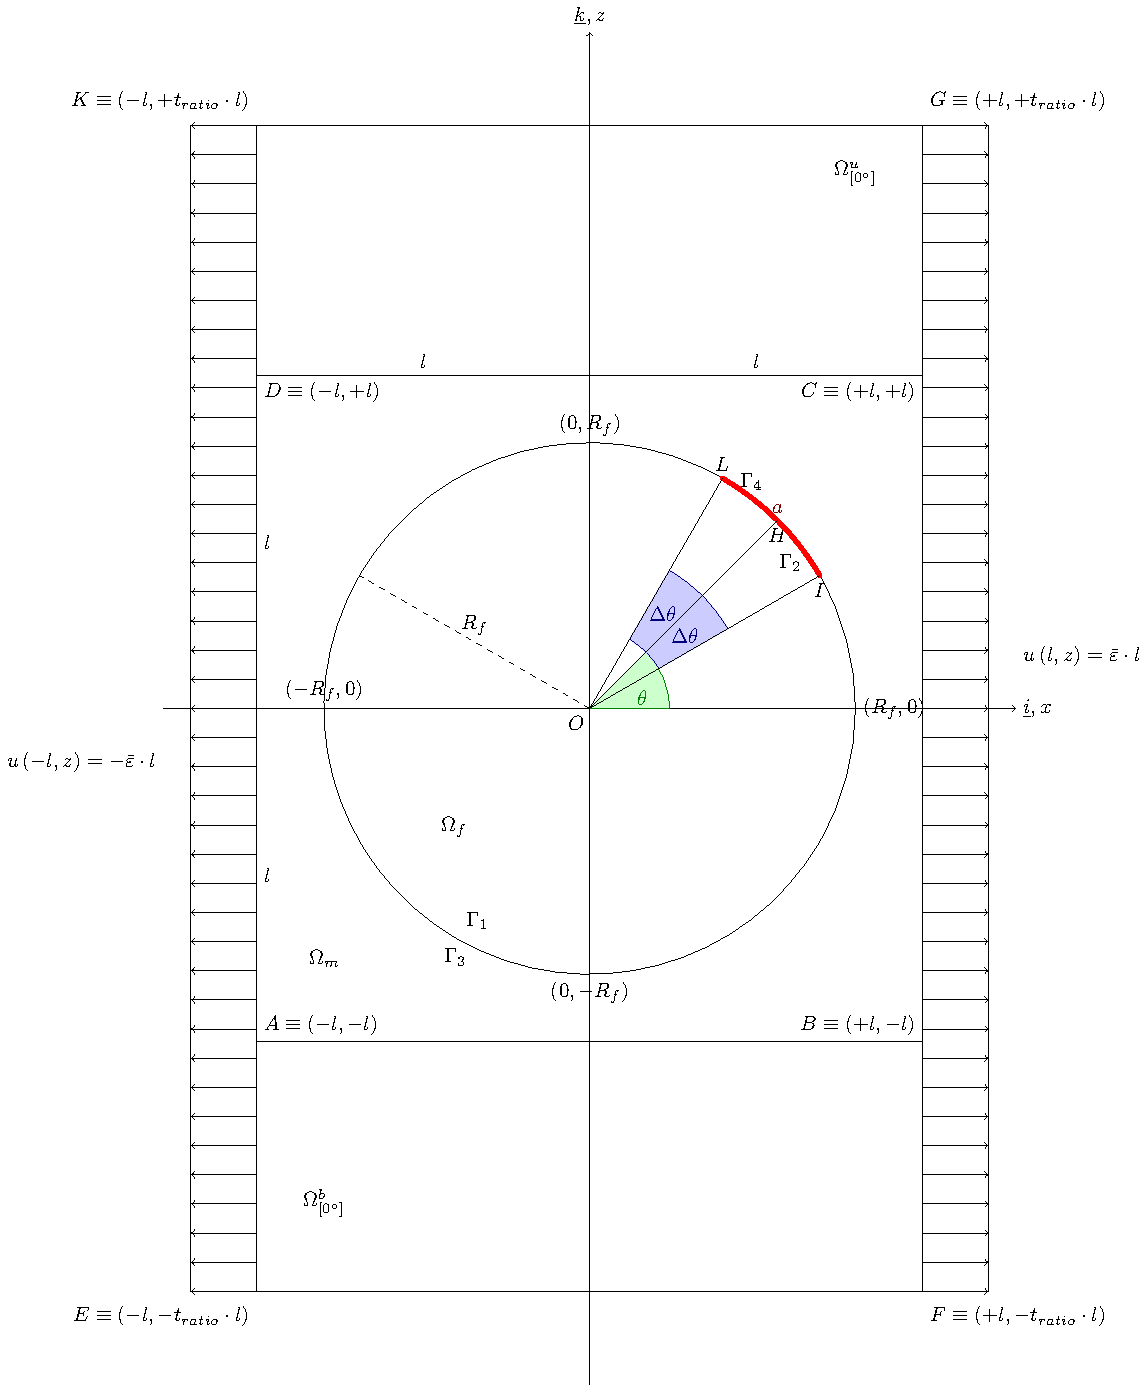
\includegraphics[height=0.275\textheight]{boundedRVE_cc.pdf}}\\
\subfloat[Periodic RVE.\label{subfig:periodic}]{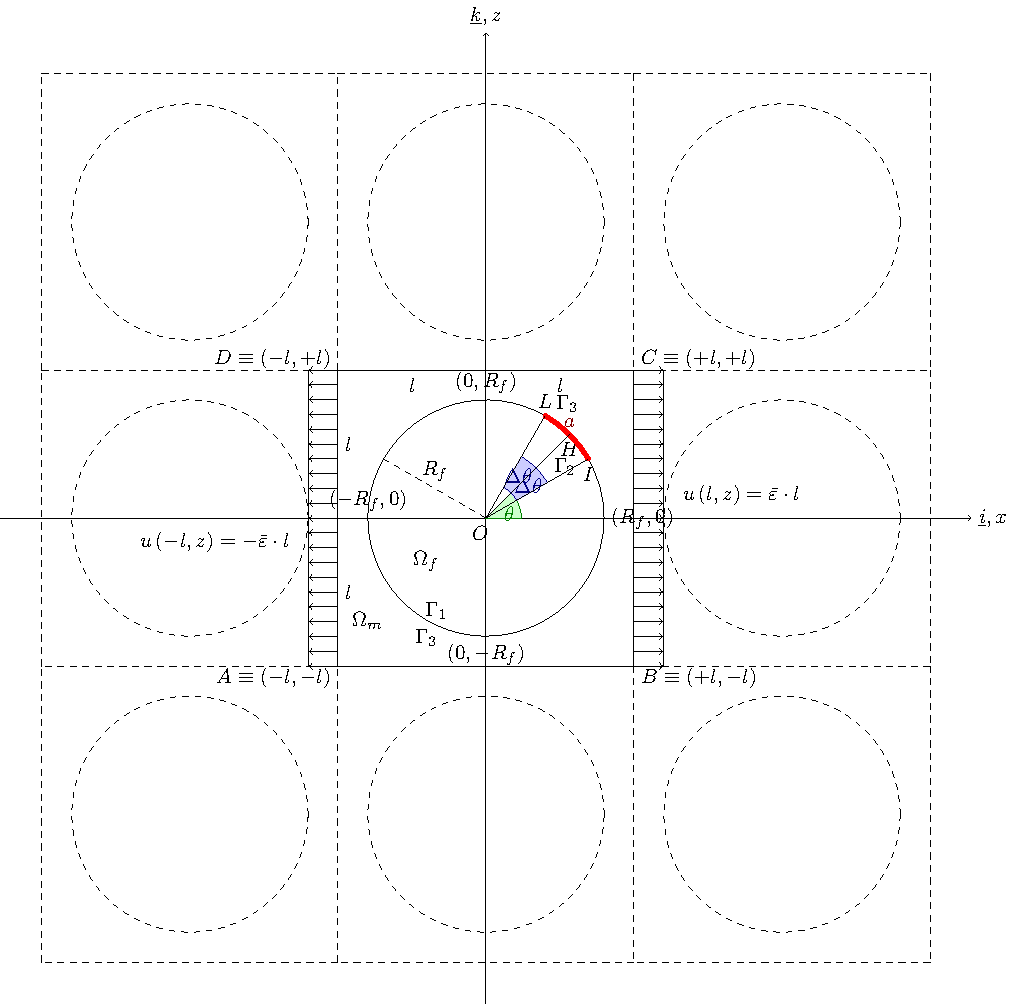
\includegraphics[height=0.275\textheight]{periodicRVE_cc.pdf}}
\caption{Representative Volume Element design: variations of boundary conditions.}
\label{fig:allRVEs}
\end{figure}
We consider the presence of a debond at the fiber/matrix interface, whose mid-arc point is placed at $\theta$ and whose angular semi-aperture with respect to the mid-point is equal to $\Delta\theta$, see Figure~\ref{subfig:free}. We evaluate the mode I, mode II and total energy release rates by means of LEFM, by employing the Virtual Crack Closure Technique (VCCT)~\cite{Krueger:2004,abaqus:2016} and J-integral evaluation ~\cite{Rice:1968,abaqus:2016}. We assume frictionless contact between crack faces and continuity constraints on the bonded part of the interface, i.e. continuity of displacements between matrix and fiber at the interface. Finally, we consider the system to be composed by two isotropic linear elastic materials: an E-glass fiber and epoxy matrix, of which properties are reported in Table~\ref{tab:phaseprop}.
\begin{table}[H]
  \centering
  \caption{Properties of E-glass fiber and epoxy matrix employed.}
    \begin{tabular}{cccc}
&&&\\
    \textbf{Material} & \textbf{$E\left[GPa\right]$}\ & \textbf{$G\left[GPa\right]$} & \textbf{$\nu\left[-\right]$} \\[3pt]
    \midrule\\[12pt]
    Glass Fiber    & 70,0  & 29,2   & 0,2  \\[16pt]
    Epoxy    & 3,5    & 1,25   & 0,4

    \end{tabular}%
  \label{tab:phaseprop}%
\end{table}%
Different variations of boundary conditions on the north and south side of the RVE are considered: free (Figure~\ref{subfig:free}); constant vertical displacement $w\left(x,\pm l\right)=w\left(l,\pm l\right)$ (Figure~\ref{subfig:homo}); homogeneous $u\left(x,\pm l\right)=\frac{x}{l}u\left(l,\pm l\right),w\left(x,\pm l\right)=w\left(l,\pm l\right)$ (Figure~\ref{subfig:homo}); bounded by the two $0^{\circ}$ plies (modeled as a homogeneous linear elastic material) (Figure~\ref{subfig:bounded}); periodicity (Figure~\ref{subfig:periodic}).
\subsection{Mesh generation and FEM model creation}
In order to apply the numerical experimentation approach previously introduced in~\ref{sub:introRVE}, a high degree of automation is required. Furthermore, the solution of Finite Elements problems is strongly dependent on the mesh, in particular for non-linear problems and in the presence of fracture processes. Thus, a software structure has been created in order to allow a controlled, categorized and automated creation of different Representative Volume Elements and Finite Elements discretization. The main elements are\footnote[1]{All the code is available under open source license at https://github.com/LucaDiStasio}: a set of mesh generation routines; a set of control routines for the parametric generation of RVEs; a Graphical User Interface.\par
Mesh generation routines have been developed in Matlab with full compatibility with its free counterpart Octave. It implements a 4-step strategy for the parametric generation of the mesh (see~\cite{ThompsonWarsiMastin:1985,ThompsonSoniWeatherill:1998} for more details):
\begin{enumerate}
\item the RVE geometry is mapped to a rectangular one by means of topological transformation, the rectangular geometry representing the computational domain of mesh generation;
\item points belonging to the boundary are generated as a set of 4 corners ($c_{i}$) and 4 edges ($e_{i}$) by using analytical parameterizations (straight lines, circles,...);
\item interior nodes are created using transfinite interpolation with multi-dimensional linear Lagrangian interpolants

\begin{equation}
r(\xi,\eta)=P_{1}(\xi,e_{2},e_{4})+P_{1}(\eta,e_{1},e_{3})- P_{2}(\xi,\eta,c_{1},c_{2},c_{3},c_{4})
\end{equation}

with

\begin{equation}
P_{1}(x,p_{j})=\sum_{j=1}^{n}p_{j}\prod_{k=1\ k\neq j}^{n}\frac{x-x_{k}}{x_{j}-x_{k}}\quad P_{2}(x,y,p_{j},q_{j})=P_{1}(x,p_{j})\otimes P_{1}(y,q_{j})
\end{equation}

where $r(\xi,\eta)$ is the position of each interior node calculated with respect to the coordinates $\xi,\eta$ in the computational domain, $p_{j}$ represents the coordinates $\left(x_{j},z_{j}\right)$ of each point on the boundary and $\otimes$ is the tensorial product.

\item The mesh is smoothed applying elliptic mesh generation

\begin{equation}
g^{11}\underline{r}_{,\xi\xi}+2g^{12}\underline{r}_{,\xi\eta}+g^{22}\underline{r}_{,\eta\eta}=0
\end{equation}

where $r$ is the position of each interior node, $\xi,\eta$ are the coordinates in the computational domain, $r_{,\cdot}$ represents derivation and $g^{ij}$ is the $i,j$ component of the $2D$ contravariant metric tensor of the mapping between physical and computational domain.
\end{enumerate}
In order to assess the effect of the mesh on FEM results, we identify the angular aperture of an element at the fiber/matrix interface $\delta$ as the parameter of reference.\par Furthermore, a transpiler to create Abaqus input files has been created in Matlab/Octave in order to convert the generated mesh into an Abaqus FEM model ready for execution.\par
Control routines are written in Python and take care of:
\begin{enumerate}
\item reading the input data provided in the form of a Comma-Separated Values (CSV) file and sort them;
\item generate the call to the preprocessor of choice (Matlab or Octave for the time being) and execute it;
\item generate the call to the FEM solver of choice (Abaqus for the time being) and execute it;
\item access the output database and perform post-processing calculations and graphics' generation.
\end{enumerate}
Finally, a GUI has been created in Mathematica for prototyping purposes, giving the possibility to visualize the different combinations of geometry and boundary conditions as well as the corresponding mesh before running the FEM simulation.
%------------------------------------------------------------------------------------------%
%                                         PRELIMINARY RESULTS
%------------------------------------------------------------------------------------------%

\section{Preliminary results}

In order to validate the strategy and the models presented, simulations have been conducted for the case of $VF_{f}\to\infty$ and $\theta=0^{\circ}$, i.e. the case of a fiber embedded in an infinite matrix with a central debond. As expected from theoretical considerations, results do not change by considering different boundary conditions. Thus, we report results only for the case of homogeneous boundary conditions (Figure~\ref{subfig:homo}) as they are representative of all cases for the fiber volume fraction considered.\par

\begin{figure}[H]
\centering
 \subfloat[$\Delta\theta=15^{\circ},$\label{subfig:traction}]{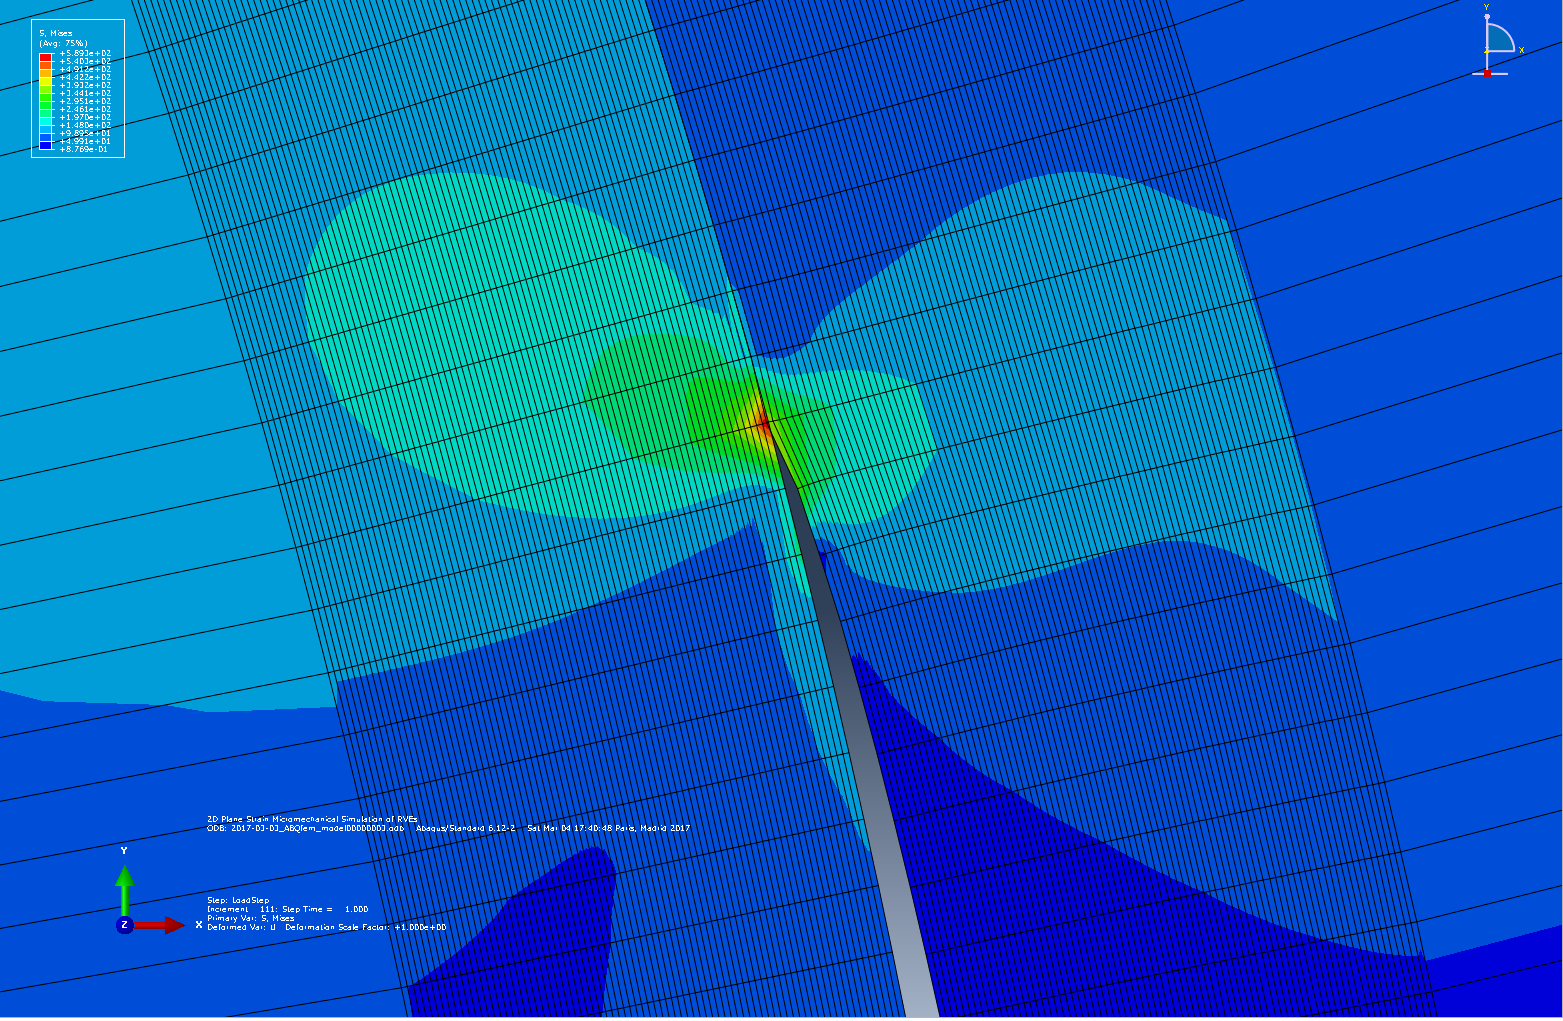
\includegraphics[width=0.475\textwidth]{abq-crack-theta-15.png}}\quad
\subfloat[$\Delta\theta=100^{\circ}$\label{subfig:shear}]{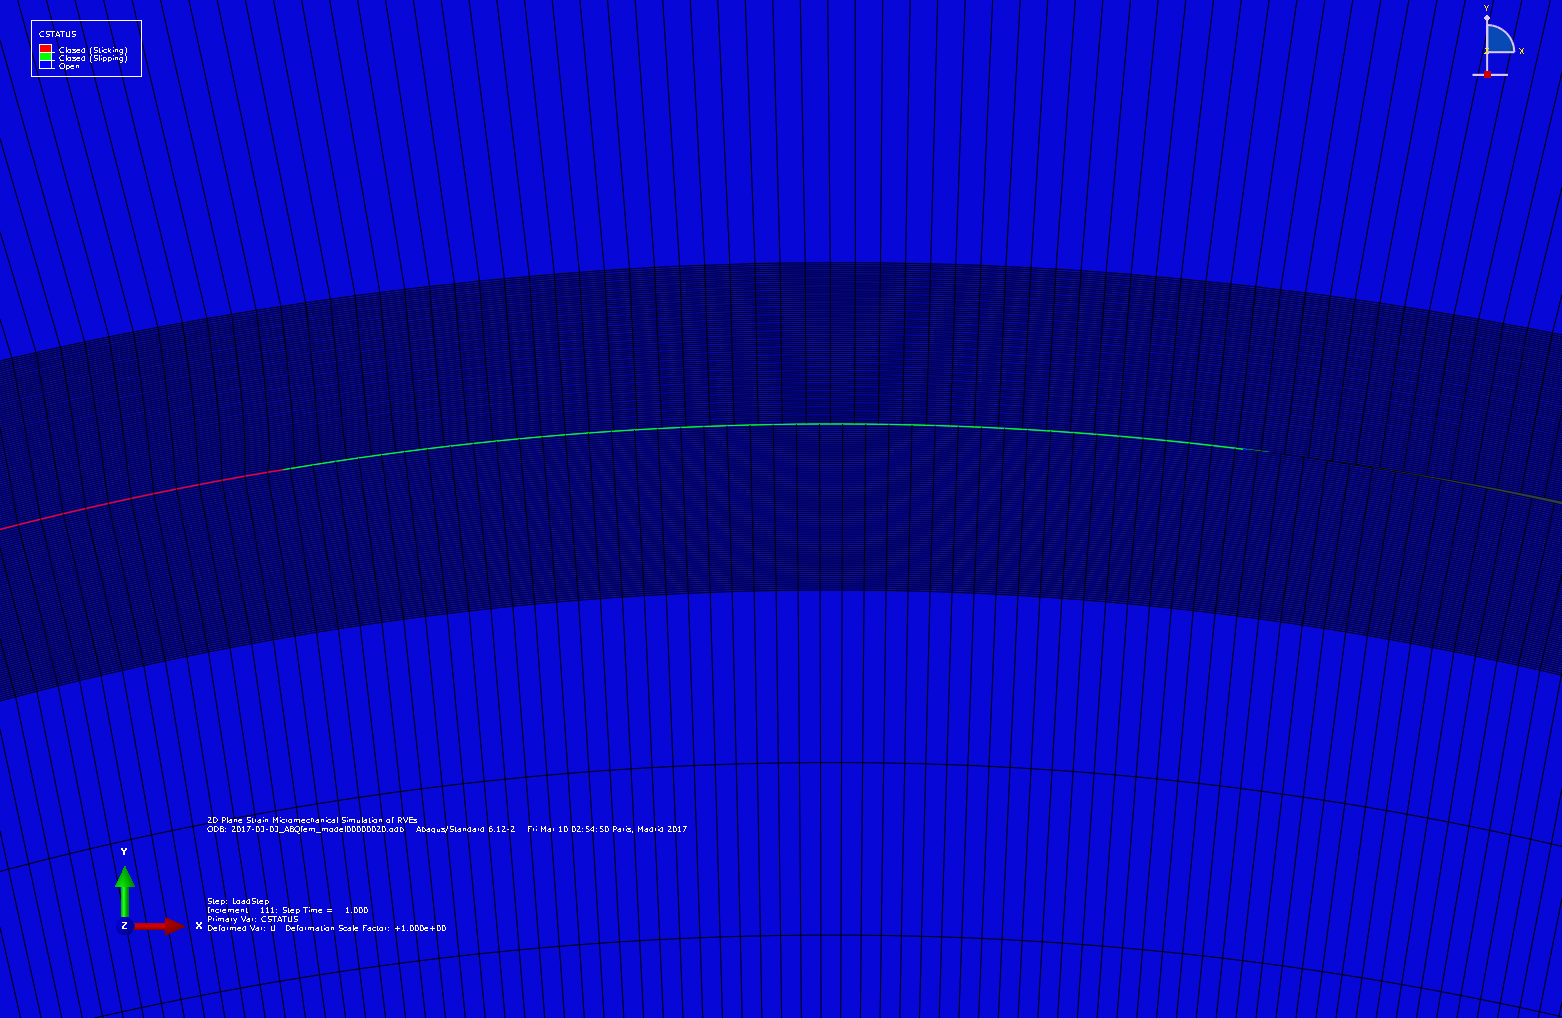
\includegraphics[width=0.475\textwidth]{abq-crack-theta-100.png}}
\caption{Numerical crack shapes for $\delta=0.4^{\circ},VF_{f}=0.001,\frac{l}{R_{f}}\approx28$.}
\label{fig:numcrackshapes}
\end{figure}

A first result to consider is the generated numerical crack shape. In Figure~\ref{fig:numcrackshapes} two different cases are reported: a first one for a debond angular semi-aperture $\Delta\Theta$ of $15^{\circ}$ (\ref{subfig:traction}) and a second for $\Delta\Theta=100^{\circ}$ (\ref{subfig:shear}). Keeping in mind that the load is applied along the $x$ direction, i.e. at $0^{\circ}$, it is possible to observe that the crack for a $15^{\circ}$ aperture is subjected almost uniquely to mode I loading. It means that traction is dominant with respect to shear in the crack opening mechanism. In the second case, mode II is the only loading mode present. In-plane shear is dominant. This is in agreement with the calculated crack shapes: for $15^{\circ}$, the crack is well open, crack faces are not in contact and stress concentration occurs at the crack tips; for $100^{\circ}$, the crack is open until $\sim70-80^{\circ}$, where crack faces come into contact and interact through shear.\par
The previous observation is in agreement with the calculated energy release rates obtained using the VCCT method in Abaqus. In Figure~\ref{fig:enrrts} the values of mode I, mode II and total energy release rates for different values of debond angular semi-aperture $\Delta\theta$. Positive values of $\Delta\theta$ correspond to crack tips in the $y>0$ plane, while negative values to crack tips in the $y<0$ plane. Thus, for each value of $\Delta\theta$ one corresponding RVE is generated and two value of energy release rates are computed, one for crack tip. Accordingly, the ratios of mode I to total energy release rate $\frac{G_{I}}{G_{I}+G_{II}}$ and the ratio of mode II to total energy release rate $\frac{G_{II}}{G_{I}+G_{II}}$ are calculated and reported in Figure~\ref{fig:moderatios}. Symmetry is evident from the two graphs, and it is in accord with the symmetry of the model studied. Furthermore, it is possible to observe how mode I is dominant for values of $\Delta\theta$ smaller than $30-40^{\circ}$; afterwards in-plane shear becomes the dominant and, for angles greater than $60-70^{\circ}$, the only crack opening mode.

\begin{figure}[H]
\centering
 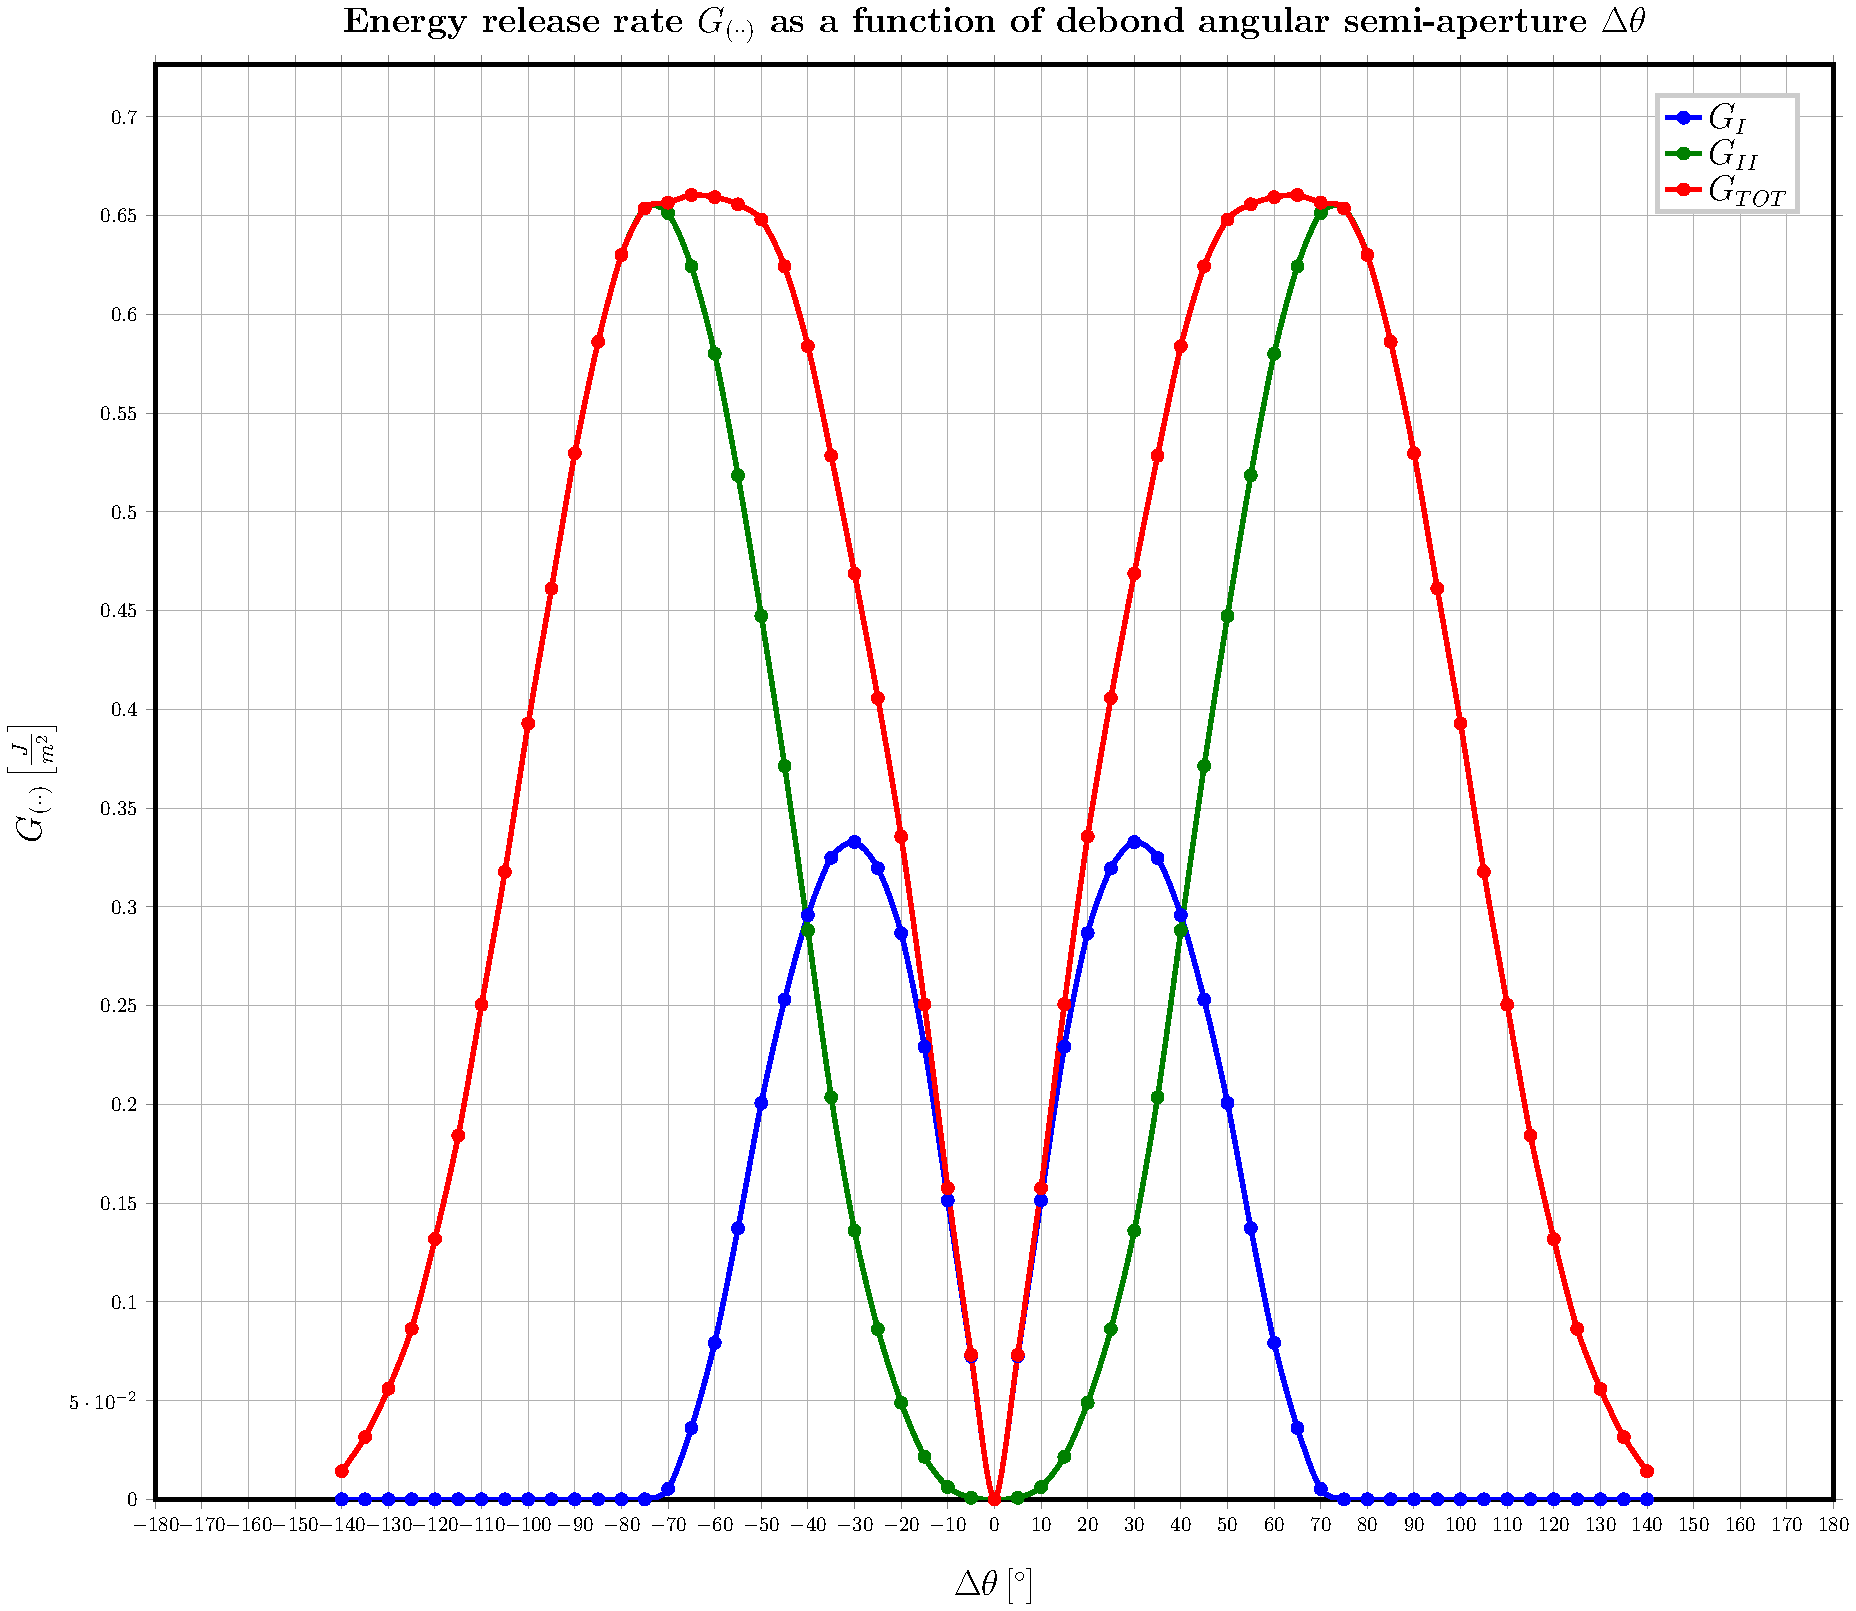
\includegraphics[height=0.45\textheight]{2017-03-03_AbqRunSummary_Gs.pdf}
 \caption{Energy release rates as a function of debond angular semi-aperture for $\delta=0.4^{\circ},VF_{f}=0.001,\frac{l}{R_{f}}\approx28$. In blue, mode I energy release rate; in green, mode II; in red, total energy release rate.}
\label{fig:enrrts}
\end{figure}

\begin{figure}[H]
\centering
 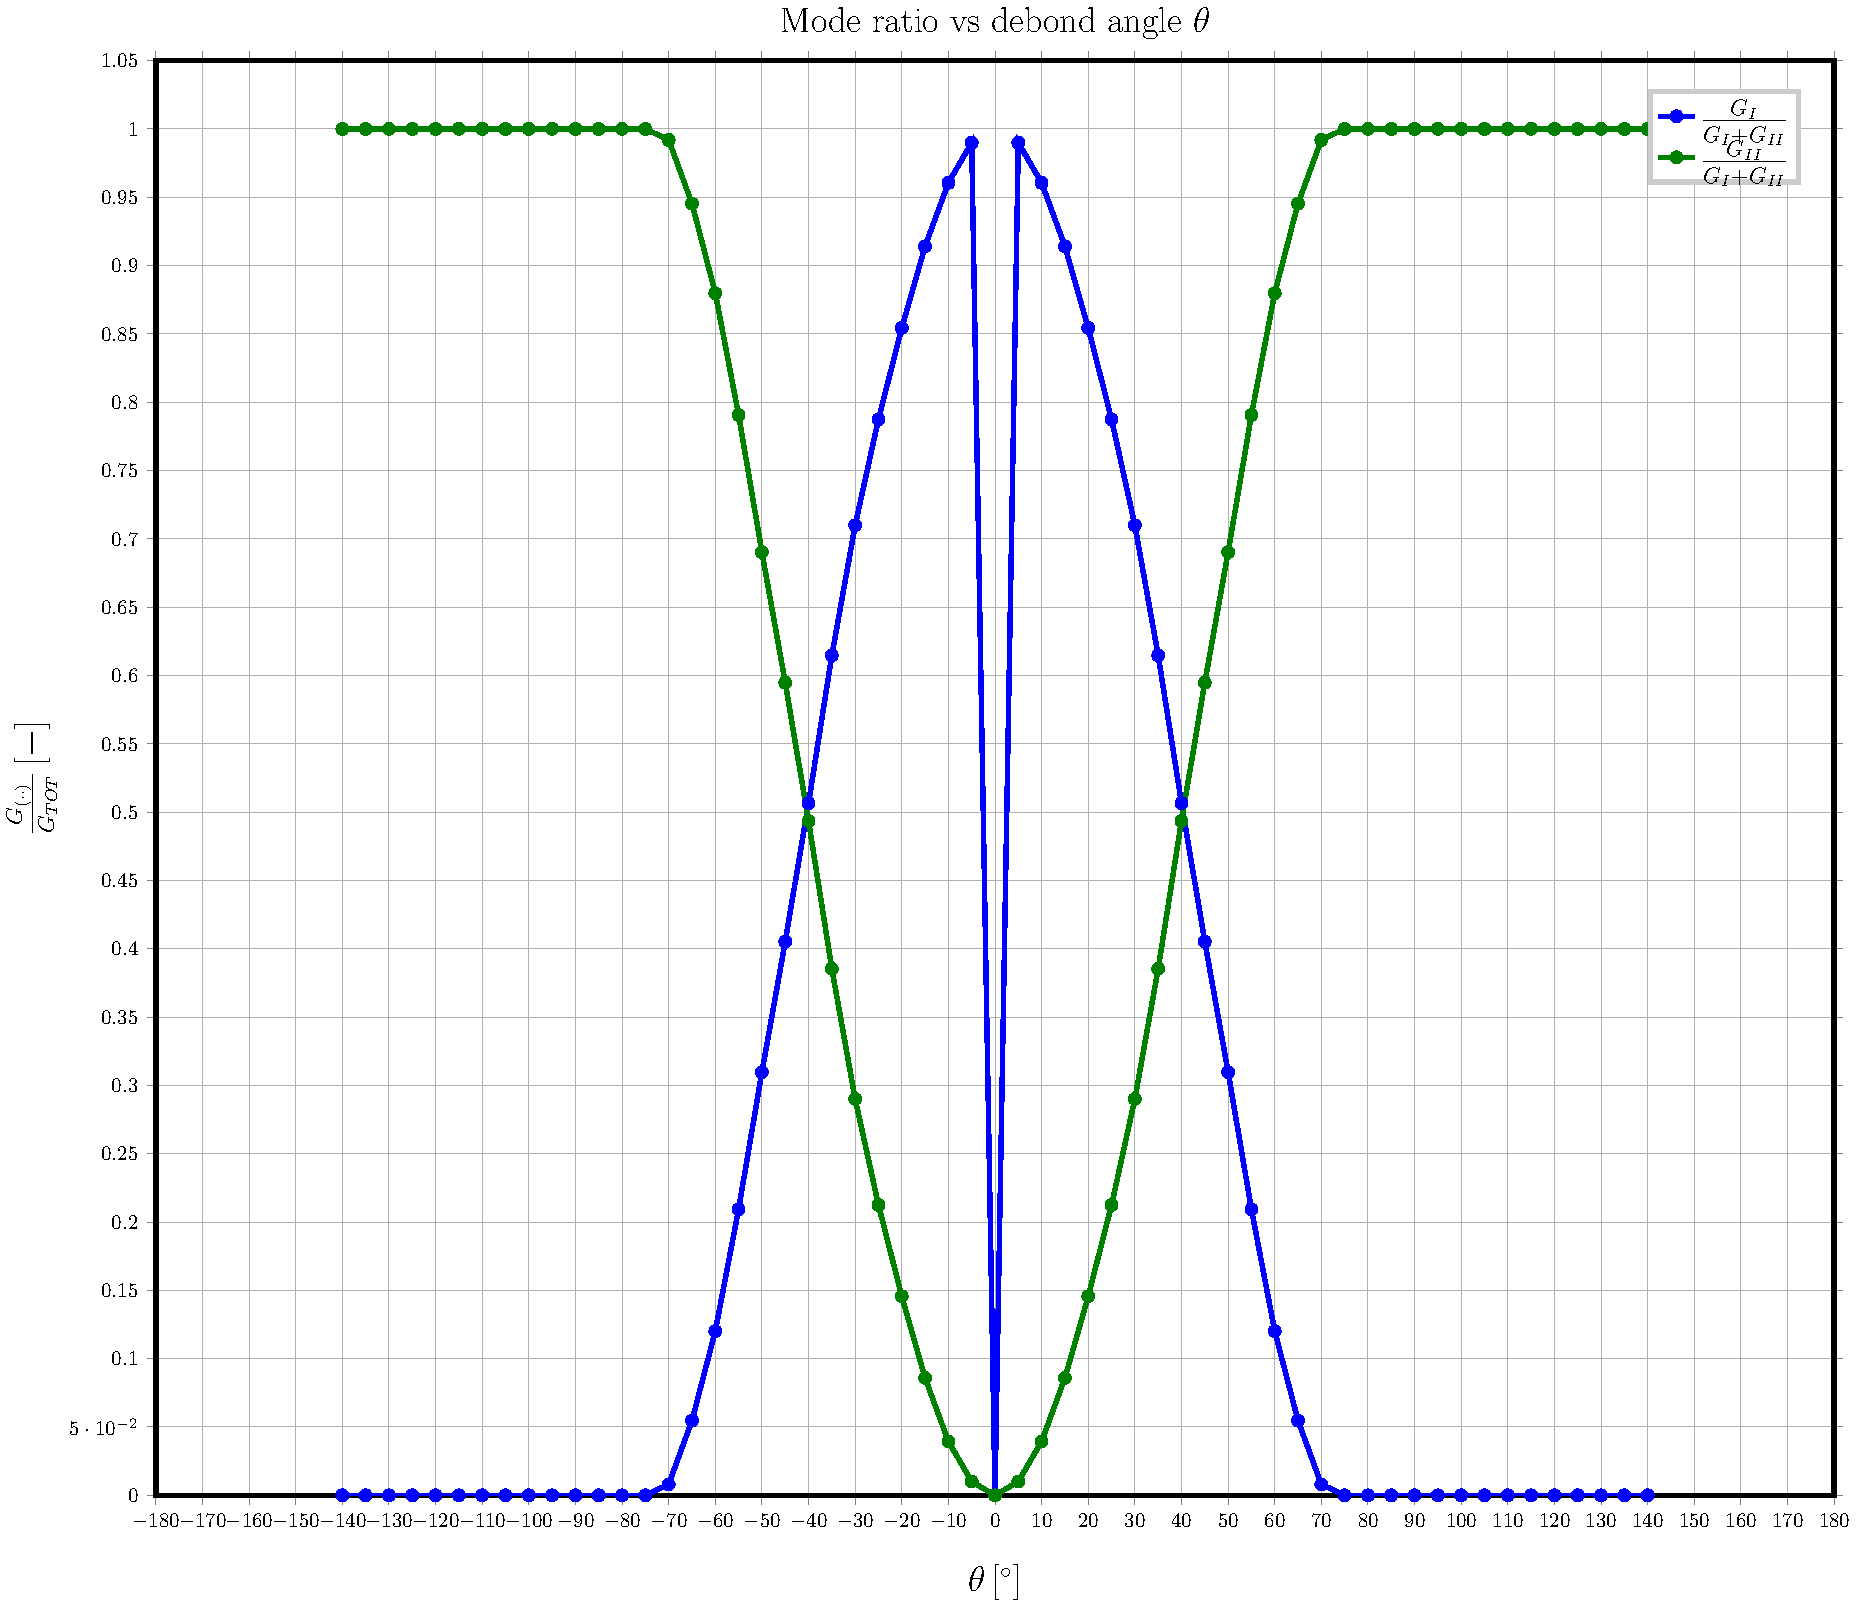
\includegraphics[height=0.45\textheight]{2017-03-03_AbqRunSummary_modeRatios.pdf}
 \caption{Mode ratio as a function of debond angular semi-aperture for $\delta=0.4^{\circ},VF_{f}=0.001,\frac{l}{R_{f}}\approx28$. In blue, ratio of mode I to total energy release rate; in green, ratio of mode II to total energy release rate.}
\label{fig:moderatios}
\end{figure}

Finally, it is interesting to analyze the performance of the FE solver (Abaqus for the present case) with respect to the mechanical parameters of the model, and in particular the debond angular semi-aperture $\Delta\Theta$. In Figure~\ref{fig:cputimes} both the total cpu time, i.e. the time spent by all the cpus, and the wall clock time, i.e. the time the user actually waits until completion, are reported. The difference between two represents the benefit provided by the use of parallelism: the smaller the wall clock time with respect to cpu time, the greater the acceleration provided by the use of parallel cores. It is possible to observe that, although present, benefits of parallelization are reduced and correspond to savings in simulation time of around $20\%$. This is due to the use of LEFM routines and the resolution of the interface. A first part of the computation is represented by LEFM evaluations, and this is the same for every value of $\Delta\theta$. The decrease in computational time with respect to $\Delta\theta$ is due to the resolution of the interface: the greater the debond, the lower the number of interface unknowns added. The time saved thanks to parallelization is related to the elastic solution of the bulk fiber and matrix: being a linear elastic problem, it can be parallelized. However, it represents only a minor part in the overall simulation, as its parallelization causes only a $20\%$ saving. Thus, the most computational expensive feature of the model is the interface: its correct modeling is important not only from the mechanical point of view, in order to evaluate correct values of energy release rate, but also from the numerical perspective, as the greatest numerical effort has to be spent on it.

\begin{figure}[H]
\centering
     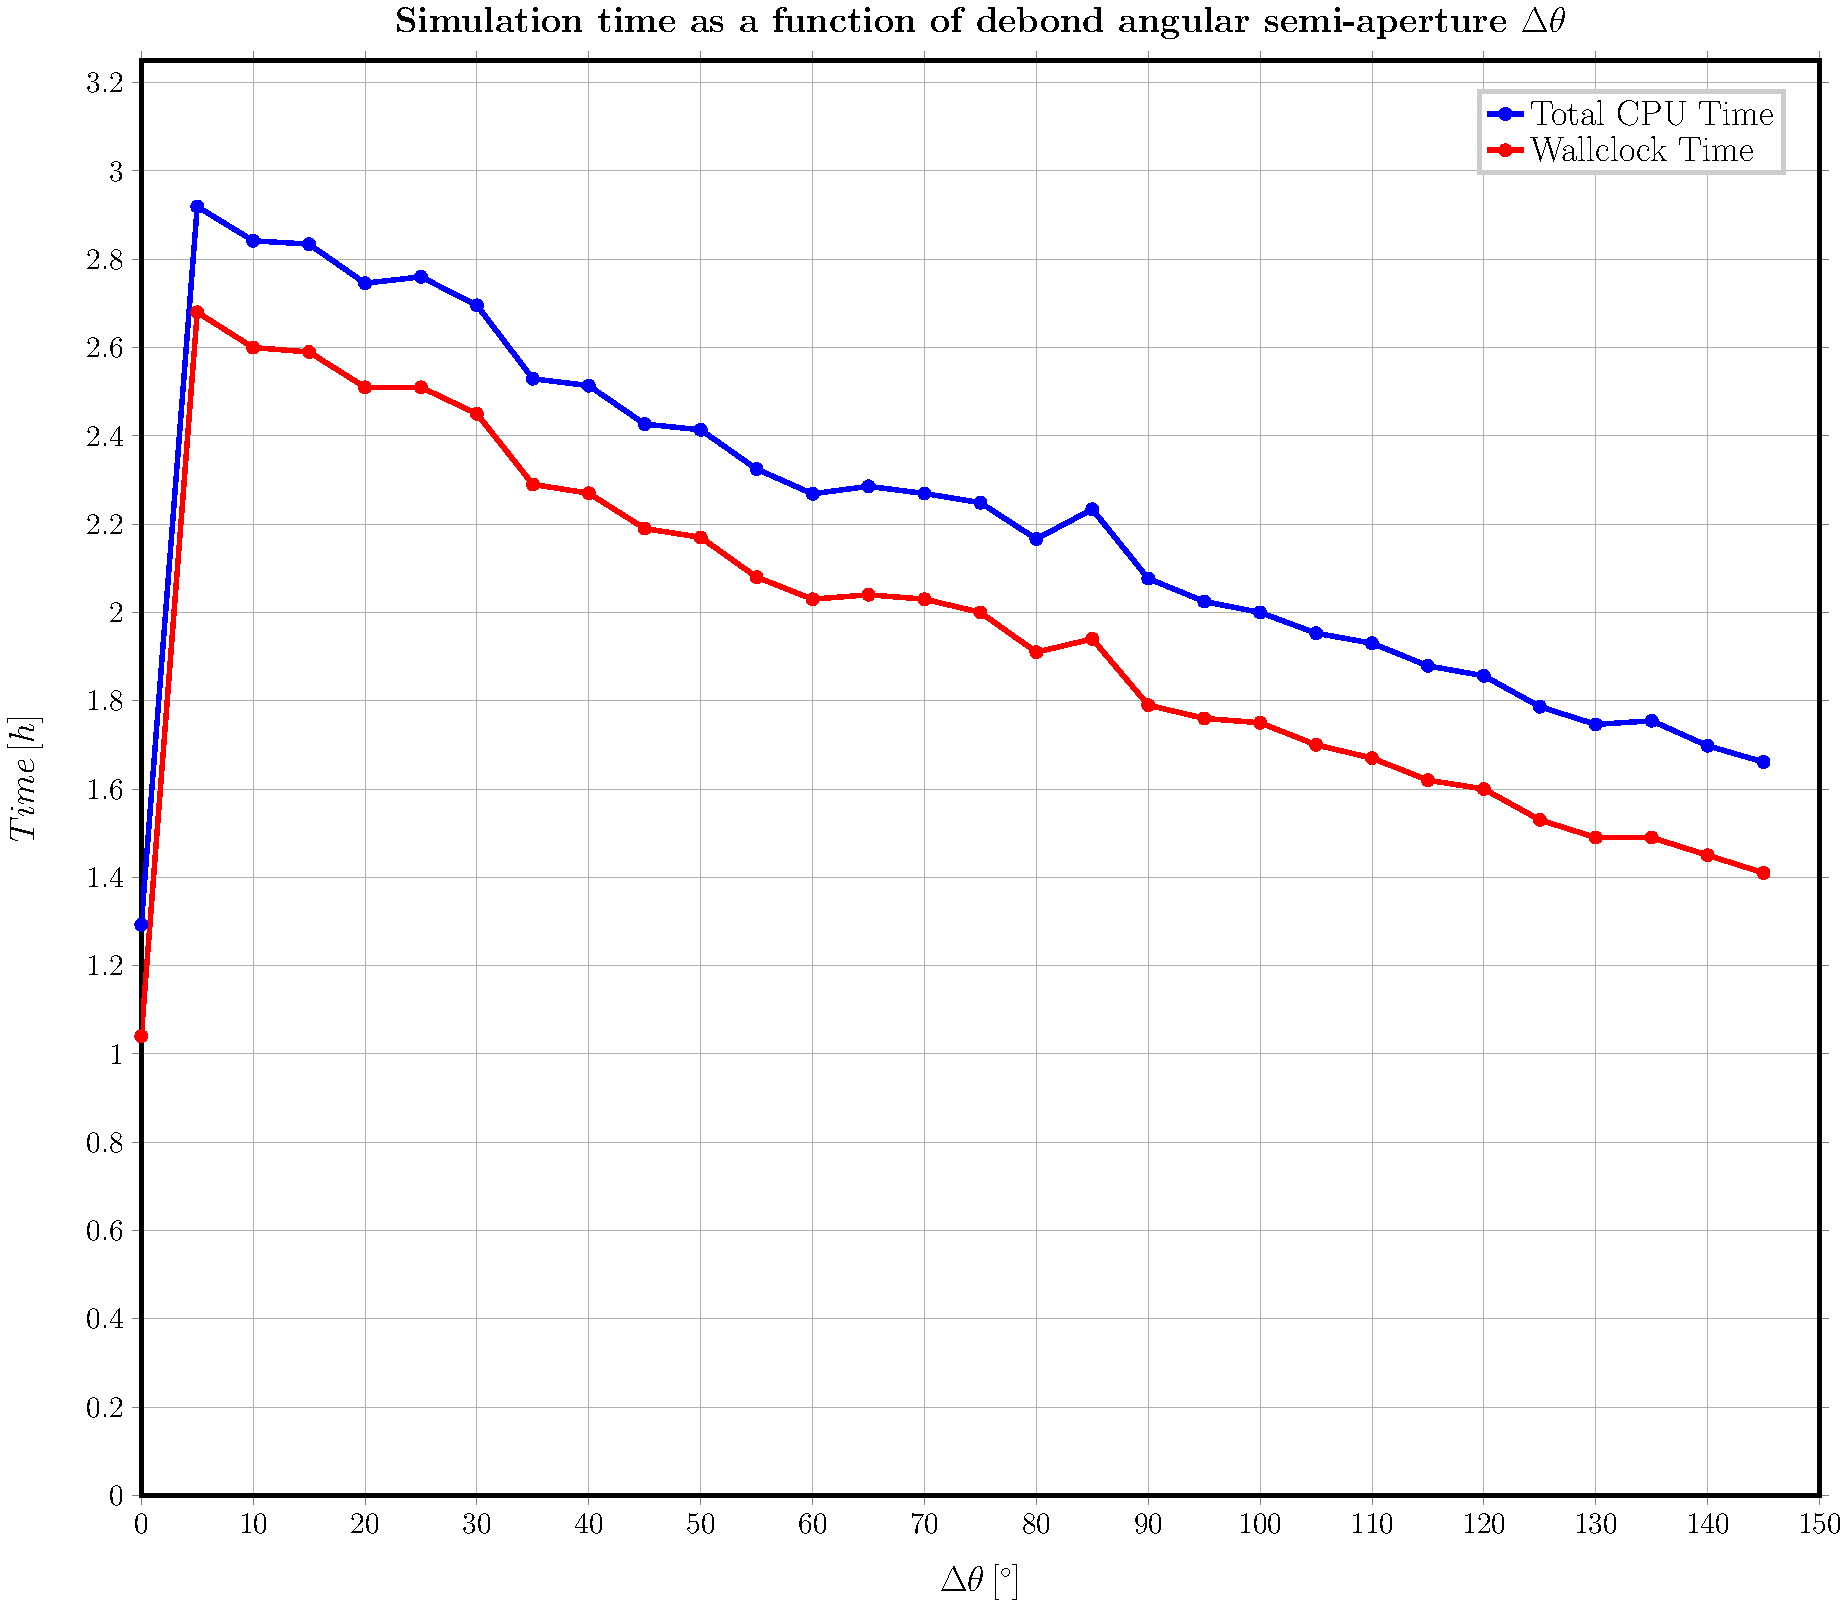
\includegraphics[height=0.45\textheight]{cpus-time.pdf}
 \caption{Cpu time and wall-clock time as a function of debond angular semi-aperture for $\delta=0.4^{\circ},VF_{f}=0.001,\frac{l}{R_{f}}\approx28$. In blue, total cpu time; in red, wall-clock time.}
\label{fig:cputimes}
\end{figure}

%------------------------------------------------------------------------------------------%
%                             CONCLUSIONS AND PERSPECTIVES
%------------------------------------------------------------------------------------------%

\section{Conclusions and Perspectives}
In order to investigate transverse crack initiation in thin ply laminates, a framework has been created for the systematic generation of different Representative Volume Elements and implemented as a set of software tools for the automatic generation and analysis of corresponding Finite Element models. A first set of models with a single fiber with its sorroundings has been tested for the case of a fiber embedded in an infinite matrix with a central debond. Results have been correctly found to be independent of the chosen boundary condition. Furthermore, crack opening has been observed to be mode I dominated for low values of $\Delta\theta$; for angles greater than $30-40^{\circ}$ mode II becomes predominant and the only one present for values greater than $60-70^{\circ}$.\par
The next steps involves the study of the dependence of energy release rate with respect to fiber volume fraction $VF_{f}$, ply thickness $t_{ply}$, debond position $\theta$, material properties and the ratio of thin ply to adjacent plies thicknesses $t_{ply}/t_{bounding\ plies}$ for the case of bounded RVE. Furthermore, the generation of new Representative Volume Elements and their categorization in a unified framework will be also the focus of future work.

%------------------------------------------------------------------------------------------%
%                                   ACKNOWLEDGEMENTS
%------------------------------------------------------------------------------------------%
\ack
Luca Di Stasio gratefully acknowledges the support of the European School of Materials (EUSMAT) through the DocMASE Doctoral Programme and the European Commission through the Erasmus Mundus Programme.
\newpage
%------------------------------------------------------------------------------------------%
%                                      REFERENCES
%------------------------------------------------------------------------------------------%
\section*{References}
\begin{thebibliography}{9}
%\bibitem{author:year}author surname author initials (up to 10) year title {\it Journal} {\bf vol} (issue) pages
% Spread Tow Technology
\bibitem{spreadtowpatent:1974}Daniels C. Pneumatic spreading of filaments. USA: Space Systems/Loral LLC; 1974. USP 3795944.
\bibitem{spreadtowpatent:1991}Iyer S., Drzal L. T. Method and system for spreading a tow of fibers. USA: Michigan State University; 1991. USP 5042122.
\bibitem{spreadtowpatent:1992}Nakagawa, N., Ohsora, Y. Fiber separator for producing fiber reinforced metallic or resin body. Japan: Ube Industries Ltd; 1992. USP 5101542.
\bibitem{spreadtowpatent:2000}Lifke J. L., Busselle L. D., Finley D. J., Gordon B. W. Method and apparatus for spreading fiber bundles. USA: Adherent Tech Inc; 2000. USP 6049956.
\bibitem{spreadtowpatent:1993}Peritt J. M., Everett R., Edelstein A. Electrostatic fiber spreader including a corona discharge device. USA: US Secretary of Navy; 1993. USP 5200620.
\bibitem{KawabeTomodaMatsuo:1997}Kawabe K., Tomoda S. and Matsuo T. 1997 A pneumatic process for spreading reinforcing fiber tow {\it Proc. 42nd Int. SAMPE USA (Anaheim, CA, USA)} 65–76.
\bibitem{spreadtowpatent:2003}Kawabe K., Tomoda S. Method of producing a spread multi-filament bundle and an apparatus used in the same. Japan: Fukui Prefectural Government; 2003. JP 2003-193895.
\bibitem{Kawabe:2008} Kawabe K. 2008 New Spreading Technology for Carbon Fiber Tow and Its Application to Composite Materials {\it Sen'i Gakkaishi} {\bf 64} (8) 262--267 [in Japanese]
\bibitem{SasayamaTomoda:2009} Sasayama H. and Tomoda S. 2009 New Carbon Fiber Tow-Spread Technology and Applications to Advanced Composite Materials {\it S.A.M.P.E. journal} {\bf 45} (2) 6--17
\bibitem{ntpt}Meijer A. NTPT makes world’s thinnest prepeg even thinner [Internet] North Thin Ply Technology (NTPT) press release 2015 [cited 30 April 2017] Available from http://www.thinplytechnology.com/mesimages/Press\_Release\_NTPT-16JUN2015.pdf
\bibitem{oxeon}oXeon TECHNOLOGIES 2014 [Internet] [cited 30 April 2017] Available from http://oxeon.se/technologies/
% Experimental studies of thin plies and/or modeling
\bibitem{SihnKimKawabeTsai:2007}Sihn S., Kim R. Y., Kawabe K. and Tsai S. W. 2007 Experimental studies of thin-ply laminated composites {\it Compos. Sci. Technol.} {\bf 67} (6) 996--1008
\bibitem{SaitoTakeuchKimpara:2012}Saito H., Takeuchi H. and Kimpara I. 2012 Experimental Evaluation of the Damage Growth Restraining in $90^{\circ}$ Layer of Thin-ply CFRP Cross-ply Laminates {\it Adv. Compos. Mater.} {\bf 21} 57--66
\bibitem{ArteiroCatalanottiXavierCamanho:2013} Arteiro A., Catalanotti G., Xavier J. and Camanho P. P. 2013 Notched response of non-crimp fabric thin-ply laminates {\it Compos. Sci. Technol.} {\bf 79} 97--114
\bibitem{AmacherCugnoniBotsisSorensenSmithDransfeld:2014}Amacher R., Cugnoni J., Botsis J., Sorensen L., Smith W. and Dransfeld C. 2014 Thin ply composites: Experimental characterization and modeling of size-effects {\it Compos. Sci. Technol.} {\bf 101} 121--132
% Thin ply effect
\bibitem{ParviziBailey:1978}Parvizi A. and Bailey J. E. 1978 On multiple transverse cracking in glass fibre epoxy cross-ply laminates {\it J Mater Sci} {\bf 13} (10) 2121--2136
\bibitem{BaileyCurtisParvizi:1979}Bailey J. E., Curtis P. T. and Parvizi A. 1979 On the Transverse Cracking and Longitudinal Splitting Behaviour of Glass and Carbon Fibre Reinforced Epoxy Cross Ply Laminates and the Effect of Poisson and Thermally Generated Strain {\it Proc. R. Soc. London, Ser. A} {\bf 366} (1727) 599--623
\bibitem{FlaggsKural:1982}Flaggs D. L. and Kural M. H. 1982 Experimental Determination of the In Situ Transverse Lamina Strength in Graphite/Epoxy Laminates {\it J. Compos. Mater.} {\bf 16} (2) 103--116
% Modeling of thin plies
\bibitem{CamanhoDavilaPinhoIannucciRobinson:2006}Camanho P. P., D\'avila C. G., Pinho S. T., Iannucci L. and Robinson P. 2006 Prediction of in situ strengths and matrix cracking in composites under transverse tension and in-plane shear {\it Composites Part A} {\bf 37} (2) 165–176
\bibitem{SaitoTakehuchiKimpara:2014}Saito H., Takehuchi H. and Kimpara I. 2014 A study of crack suppression mechanism of thin-ply carbon-fiber-reinforced polymer laminate with mesoscopic numerical simulation {\it J. Compos. Mater.} {\bf 48} (17) 2085 - 2096
\bibitem{HerraezMoraNayaLopesGonzalezLLorca:2015}Herr\'aez M., Mora D., Naya F., Lopes C. S., Gonz\'alez C. and LLorca J. 2015 Transverse cracking of cross-ply laminates: A computational micromechanics perspective {\it Compos. Sci. Technol.} {\bf 110} 196--204
\bibitem{CanalGonzalezSeguradoLLorca:2012}Canal L. P., Gonz\'alez C., Segurado J. and LLorca J. 2012 Intraply fracture of fiber-reinforced composites: Microscopic mechanisms and modeling {\it Compos. Sci. Technol.} {\bf 72} (11) 1223--1232
% Representative Volume Element
\bibitem{Hill:1963}Hill R. 1963 Elastic properties of reinforced solids: Some theoretical principles {\it J. Mech. Ph. Solids} {\bf 11} (5) 357--372
\bibitem{SunVaidya:1996}Sun C. T. and Vaidya R. S. 1996 Prediction of composite properties from a representative volume element {\it Compos. Sci. Technol.} {\bf 56} (2) 171--179
\bibitem{Hashin:1983}Hashin Z. 1983 Analysis of Composite Materials -- A Survey {\it J. Appl. Mech} {\bf 50} (3) 481--505
\bibitem{Hashin:1962}Hashin Z. 1962 On some variational principles in anisotropic and nonhomogeneous elasticity {\it J. Mech. Ph. Solids} {\bf 10} (4) 335--342
\bibitem{Hashin:1963}Hashin Z. 1963 A variational approach to the theory of the elastic behaviour of multiphase materials {\it J. Mech. Ph. Solids} {\bf 11} (2) 127--140
\bibitem{SwaminathanGhoshPagano:2006}Swaminathan S., Ghosh S. and Pagano N. J. 2006 Statistically Equivalent Representative Volume Elements for Unidirectional Composite Microstructures: Part I - Without Damage {\it J. Compos. Mater.} {\bf 40} (7) 583--604
\bibitem{SwaminathanGhosh:2006}Swaminathan S.and Ghosh S. 2006 Statistically Equivalent Representative Volume Elements for Unidirectional Composite Microstructures: Part II - With Interfacial Debonding {\it J. Compos. Mater.} {\bf 40} (7) 605--621
\bibitem{BulsaraTalrejaQu:1999}Bulsara V. N., Talreja R. and Qu J. 1999 Damage initiation under transverse loading of unidirectional composites with arbitrarily distributed fibers {\it Compos. Sci. Technol.} {\bf 59} (5) 673--682
\bibitem{Krauth:2009}Krauth W. 2009 Four lectures on computational statistical physics {\it eprint arXiv:0901.2496} Available from https://arxiv.org/abs/0901.2496.
\bibitem{HoffmannSchreiber:2002}Hoffmann K. H. and Schreiber M. 2002 {\it Computational Statistical Physics} (Berlin: Springer)
% LEFM
\bibitem{Krueger:2004}Krueger R. 2004 Virtual crack closure technique: History, approach, and applications {\it Appl. Mech. Rev.} {\bf 57} (2) 109--143
\bibitem{abaqus:2016} ABAQUS 2016 ABAQUS 2016 Analysis User's Manual {\it Online Documentation Help: Dassault Syst\'emes} 
\bibitem{Rice:1968}Rice J. R. 1968 A Path Independent Integral and the Approximate Analysis of Strain Concentration by Notches and Cracks {\it J. Appl. Mech.} {\bf 35} 379--386
% Mesh generation
\bibitem{ThompsonWarsiMastin:1985}Thompson J. F., Warsi Z. U. A. and Mastin C. W. 1985 {\it Numerical Grid Generation} (Elsevier Science Publishing Co.)
\bibitem{ThompsonSoniWeatherill:1998}Thompson J. F., Soni B. K. and Weatherill N. P. 1998 {\it Handbook of Grid Generation} (CRC Press)
%\bibitem{author:year}
\end{thebibliography}

%------------------------------------------------------------------------------------------%
%------------------------------------------------------------------------------------------%
%                                    DOCUMENT ENDS
%------------------------------------------------------------------------------------------%
%------------------------------------------------------------------------------------------%
\end{document}

%------------------------------------------------------------------------------------------%
%------------------------------------------------------------------------------------------%
%------------------------------------------------------------------------------------------%
%                                      FILE ENDS
%------------------------------------------------------------------------------------------%
%------------------------------------------------------------------------------------------%
%------------------------------------------------------------------------------------------%
